\documentclass{article}
\usepackage{tikz}
\usepackage{tikz-qtree}
\begin{document}
\section{Trees}


Shifting one case:


\bigskip

[1, 1, 1, 1, 1, 1, 1, 1, 1, 1, 0, 0, 0, 0, 0, 0, 0, 1, 1, 0, 1, 0, 1, 1, 0, 1, 0, 0, 0, 1, 0, 1, 0, 1, 1, 1, 1, 0, 0, 0, 0, 1, 0, 1, 1, 1, 1, 0, 1, 0, 1, 0, 0, 0, 0, 0, 0, 0, 1, 0, 1, 0]


\begin{tikzpicture}[every tree node/.style={draw,circle},sibling distance=10pt, level distance=40pt]
\tikzset{edge from parent/.style={draw, edge from parent path=
    {(\tikzparentnode) -- (\tikzchildnode)}}}
    \Tree [.3 [.1 [.1 [.P(7) [.L(1) [.1 [.1 [.1 [.1 [.1 [.0 ] ] ] ] ] ] ] [.O(3) [.0 ] [.0 ] [.2 [.0 ] [.0 ] ] ] [.0 ] [.0 ] [.1 [.1 [.1 [.0 ] ] ] ] [.0 ] [.1 [.1 [.3 [.0 ] [.0 ] [.0 ] ] ] ] ] ] ] [.0 ] [.0 ] ] 
\end{tikzpicture}

[1, 1, 1, 1, 1, 1, 1, 1, 1, 1, 1, 0, 0, 0, 0, 0, 0, 0, 1, 0, 1, 0, 1, 1, 0, 1, 0, 0, 0, 1, 0, 1, 0, 1, 1, 1, 1, 0, 0, 0, 0, 1, 0, 1, 1, 1, 1, 0, 1, 0, 1, 0, 0, 0, 0, 0, 0, 0, 1, 0, 1, 0]


\begin{tikzpicture}[every tree node/.style={draw,circle},sibling distance=10pt, level distance=40pt]
\tikzset{edge from parent/.style={draw, edge from parent path=
    {(\tikzparentnode) -- (\tikzchildnode)}}}
    \Tree [.3 [.1 [.1 [.P(6) [.O(4) [.L(1) [.1 [.1 [.1 [.1 [.1 [.0 ] ] ] ] ] ] ] [.0 ] [.0 ] [.2 [.0 ] [.0 ] ] ] [.0 ] [.0 ] [.1 [.1 [.1 [.0 ] ] ] ] [.0 ] [.1 [.1 [.3 [.0 ] [.0 ] [.0 ] ] ] ] ] ] ] [.0 ] [.0 ] ] 
\end{tikzpicture}






\bigskip






\bigskip



--------------------------------------------------------------


\bigskip






\bigskip



Shifting zero case:


\bigskip

[1, 1, 1, 1, 1, 1, 1, 1, 0, 0, 0, 0, 1, 0, 1, 1, 0, 1, 0, 0, 1, 0, 1, 1, 1, 0, 0, 0, 1, 0, 0, 1, 0, 1, 0, 1, 0, 0, 0, 1, 0, 1, 0, 0, 1, 0, 1, 0, 1, 0]


\begin{tikzpicture}[every tree node/.style={draw,circle},sibling distance=10pt, level distance=40pt]
\tikzset{edge from parent/.style={draw, edge from parent path=
    {(\tikzparentnode) -- (\tikzchildnode)}}}
    \Tree [.4 [.3 [.1 [.4 [.P(6) [.L(1) [.1 [.1 [.0 ] ] ] ] [.O(0) ] [.2 [.0 ] [.0 ] ] [.0 ] [.1 [.1 [.0 ] ] ] [.0 ] ] [.0 ] [.0 ] [.0 ] ] ] [.0 ] [.0 ] ] [.0 ] [.0 ] [.0 ] ] 
\end{tikzpicture}

[1, 0, 1, 1, 1, 1, 1, 1, 1, 0, 0, 0, 0, 1, 1, 1, 0, 1, 0, 0, 1, 0, 1, 1, 1, 0, 0, 0, 1, 0, 0, 1, 0, 1, 0, 1, 0, 0, 0, 1, 0, 1, 0, 0, 1, 0, 1, 0, 1, 0]


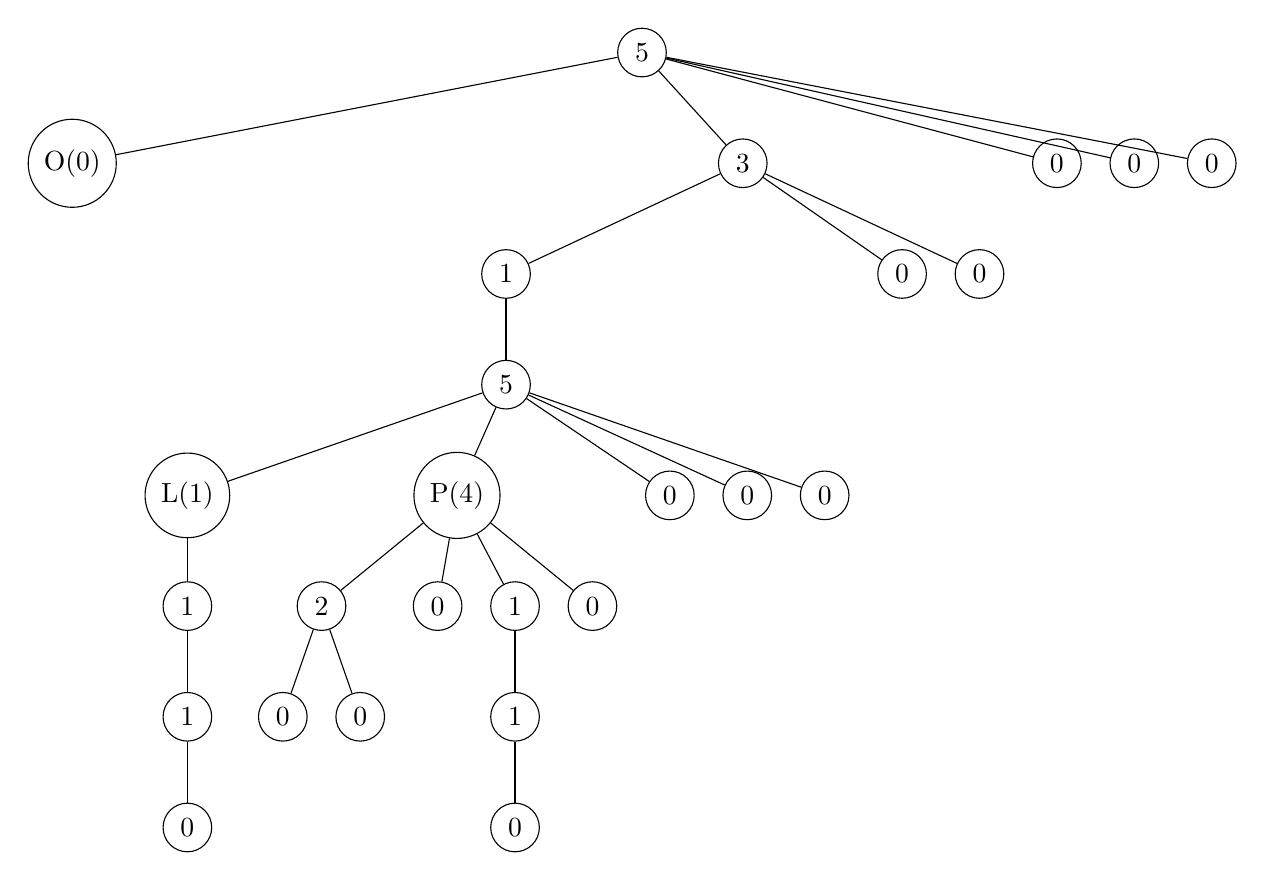
\begin{tikzpicture}[every tree node/.style={draw,circle},sibling distance=10pt, level distance=40pt]
\tikzset{edge from parent/.style={draw, edge from parent path=
    {(\tikzparentnode) -- (\tikzchildnode)}}}
    \Tree [.5 [.O(0) ] [.3 [.1 [.5 [.L(1) [.1 [.1 [.0 ] ] ] ] [.P(4) [.2 [.0 ] [.0 ] ] [.0 ] [.1 [.1 [.0 ] ] ] [.0 ] ] [.0 ] [.0 ] [.0 ] ] ] [.0 ] [.0 ] ] [.0 ] [.0 ] [.0 ] ] 
\end{tikzpicture}



---------------------


\bigskip



Tight case 


\bigskip

[1, 1, 1, 0, 0, 0, 1, 0, 1, 0, 1, 0, 1, 0, 1, 0, 1, 0, 1, 0]


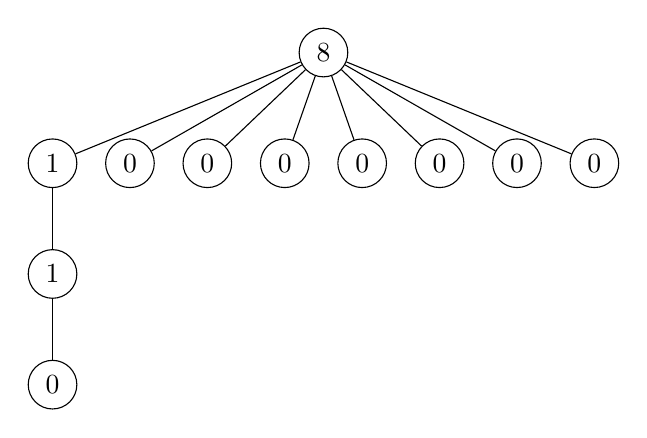
\begin{tikzpicture}[every tree node/.style={draw,circle},sibling distance=10pt, level distance=40pt]
\tikzset{edge from parent/.style={draw, edge from parent path=
    {(\tikzparentnode) -- (\tikzchildnode)}}}
    \Tree [.8 [.1 [.1 [.0 ] ] ] [.0 ] [.0 ] [.0 ] [.0 ] [.0 ] [.0 ] [.0 ] ] 
\end{tikzpicture}

[1, 1, 1, 1, 0, 0, 0, 0, 1, 0, 1, 0, 1, 0, 1, 0, 1, 0, 1, 0]





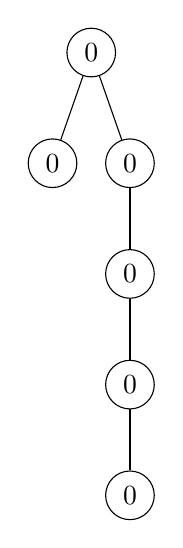
\begin{tikzpicture}[every tree node/.style={draw,circle},sibling distance=10pt, level distance=40pt]
\tikzset{edge from parent/.style={draw, edge from parent path=
{(\tikzparentnode) -- (\tikzchildnode)}}}
\Tree[.0 [.0 ] [.0 [.0 [.0 [.0 ] ] ] ] ] 
\end{tikzpicture}

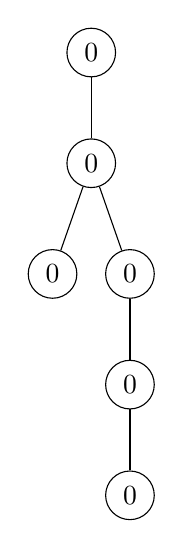
\begin{tikzpicture}[every tree node/.style={draw,circle},sibling distance=10pt, level distance=40pt]
\tikzset{edge from parent/.style={draw, edge from parent path=
{(\tikzparentnode) -- (\tikzchildnode)}}}
\Tree[.0 [.0 [.0 ] [.0 [.0 [.0 ] ] ] ] ] 
\end{tikzpicture}

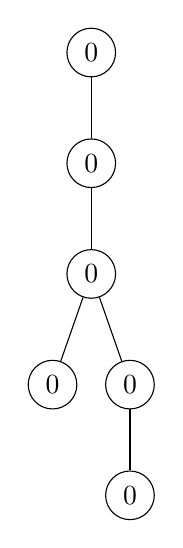
\begin{tikzpicture}[every tree node/.style={draw,circle},sibling distance=10pt, level distance=40pt]
\tikzset{edge from parent/.style={draw, edge from parent path=
{(\tikzparentnode) -- (\tikzchildnode)}}}
\Tree[.0 [.0 [.0 [.0 ] [.0 [.0 ] ] ] ] ] 
\end{tikzpicture}

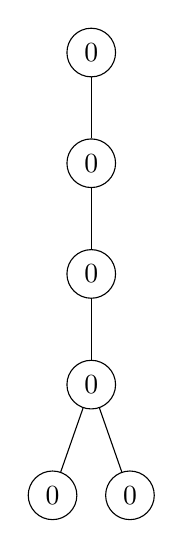
\begin{tikzpicture}[every tree node/.style={draw,circle},sibling distance=10pt, level distance=40pt]
\tikzset{edge from parent/.style={draw, edge from parent path=
{(\tikzparentnode) -- (\tikzchildnode)}}}
\Tree[.0 [.0 [.0 [.0 [.0 ] [.0 ] ] ] ] ] 
\end{tikzpicture}

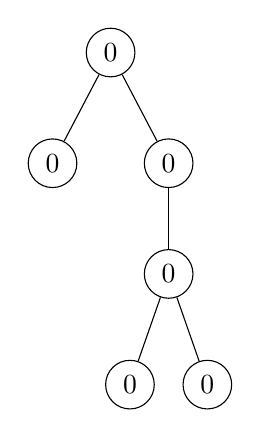
\begin{tikzpicture}[every tree node/.style={draw,circle},sibling distance=10pt, level distance=40pt]
\tikzset{edge from parent/.style={draw, edge from parent path=
{(\tikzparentnode) -- (\tikzchildnode)}}}
\Tree[.0 [.0 ] [.0 [.0 [.0 ] [.0 ] ] ] ] 
\end{tikzpicture}

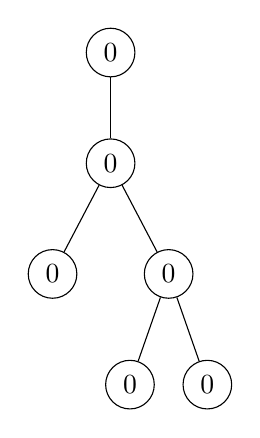
\begin{tikzpicture}[every tree node/.style={draw,circle},sibling distance=10pt, level distance=40pt]
\tikzset{edge from parent/.style={draw, edge from parent path=
{(\tikzparentnode) -- (\tikzchildnode)}}}
\Tree[.0 [.0 [.0 ] [.0 [.0 ] [.0 ] ] ] ] 
\end{tikzpicture}

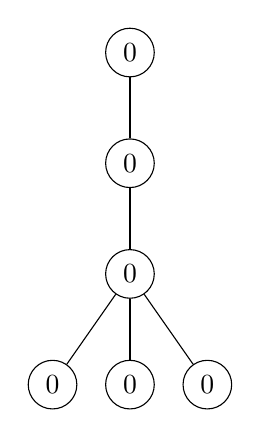
\begin{tikzpicture}[every tree node/.style={draw,circle},sibling distance=10pt, level distance=40pt]
\tikzset{edge from parent/.style={draw, edge from parent path=
{(\tikzparentnode) -- (\tikzchildnode)}}}
\Tree[.0 [.0 [.0 [.0 ] [.0 ] [.0 ] ] ] ] 
\end{tikzpicture}

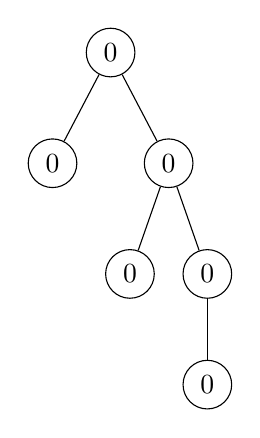
\begin{tikzpicture}[every tree node/.style={draw,circle},sibling distance=10pt, level distance=40pt]
\tikzset{edge from parent/.style={draw, edge from parent path=
{(\tikzparentnode) -- (\tikzchildnode)}}}
\Tree[.0 [.0 ] [.0 [.0 ] [.0 [.0 ] ] ] ] 
\end{tikzpicture}

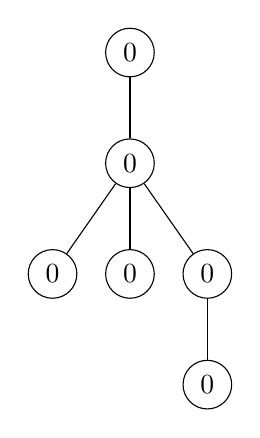
\begin{tikzpicture}[every tree node/.style={draw,circle},sibling distance=10pt, level distance=40pt]
\tikzset{edge from parent/.style={draw, edge from parent path=
{(\tikzparentnode) -- (\tikzchildnode)}}}
\Tree[.0 [.0 [.0 ] [.0 ] [.0 [.0 ] ] ] ] 
\end{tikzpicture}

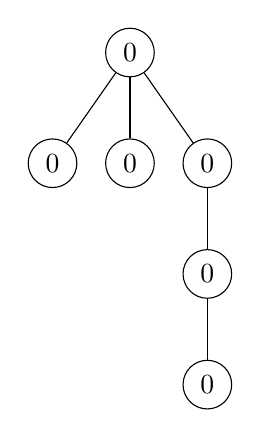
\begin{tikzpicture}[every tree node/.style={draw,circle},sibling distance=10pt, level distance=40pt]
\tikzset{edge from parent/.style={draw, edge from parent path=
{(\tikzparentnode) -- (\tikzchildnode)}}}
\Tree[.0 [.0 ] [.0 ] [.0 [.0 [.0 ] ] ] ] 
\end{tikzpicture}

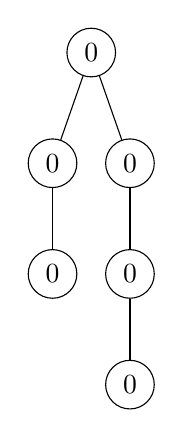
\begin{tikzpicture}[every tree node/.style={draw,circle},sibling distance=10pt, level distance=40pt]
\tikzset{edge from parent/.style={draw, edge from parent path=
{(\tikzparentnode) -- (\tikzchildnode)}}}
\Tree[.0 [.0 [.0 ] ] [.0 [.0 [.0 ] ] ] ] 
\end{tikzpicture}

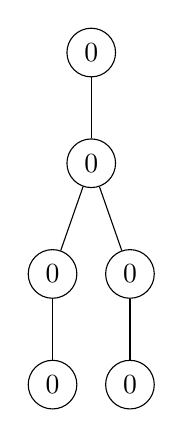
\begin{tikzpicture}[every tree node/.style={draw,circle},sibling distance=10pt, level distance=40pt]
\tikzset{edge from parent/.style={draw, edge from parent path=
{(\tikzparentnode) -- (\tikzchildnode)}}}
\Tree[.0 [.0 [.0 [.0 ] ] [.0 [.0 ] ] ] ] 
\end{tikzpicture}

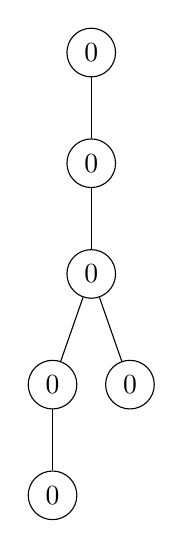
\begin{tikzpicture}[every tree node/.style={draw,circle},sibling distance=10pt, level distance=40pt]
\tikzset{edge from parent/.style={draw, edge from parent path=
{(\tikzparentnode) -- (\tikzchildnode)}}}
\Tree[.0 [.0 [.0 [.0 [.0 ] ] [.0 ] ] ] ] 
\end{tikzpicture}

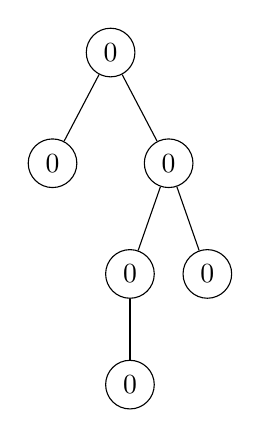
\begin{tikzpicture}[every tree node/.style={draw,circle},sibling distance=10pt, level distance=40pt]
\tikzset{edge from parent/.style={draw, edge from parent path=
{(\tikzparentnode) -- (\tikzchildnode)}}}
\Tree[.0 [.0 ] [.0 [.0 [.0 ] ] [.0 ] ] ] 
\end{tikzpicture}

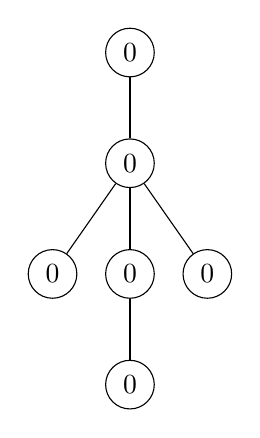
\begin{tikzpicture}[every tree node/.style={draw,circle},sibling distance=10pt, level distance=40pt]
\tikzset{edge from parent/.style={draw, edge from parent path=
{(\tikzparentnode) -- (\tikzchildnode)}}}
\Tree[.0 [.0 [.0 ] [.0 [.0 ] ] [.0 ] ] ] 
\end{tikzpicture}

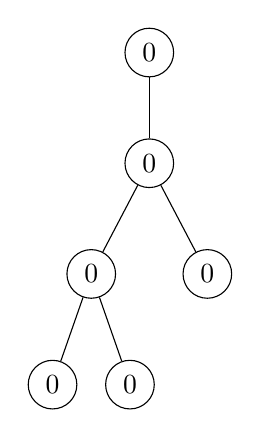
\begin{tikzpicture}[every tree node/.style={draw,circle},sibling distance=10pt, level distance=40pt]
\tikzset{edge from parent/.style={draw, edge from parent path=
{(\tikzparentnode) -- (\tikzchildnode)}}}
\Tree[.0 [.0 [.0 [.0 ] [.0 ] ] [.0 ] ] ] 
\end{tikzpicture}

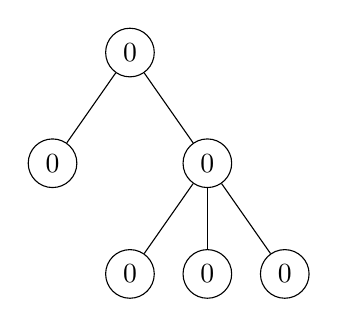
\begin{tikzpicture}[every tree node/.style={draw,circle},sibling distance=10pt, level distance=40pt]
\tikzset{edge from parent/.style={draw, edge from parent path=
{(\tikzparentnode) -- (\tikzchildnode)}}}
\Tree[.0 [.0 ] [.0 [.0 ] [.0 ] [.0 ] ] ] 
\end{tikzpicture}

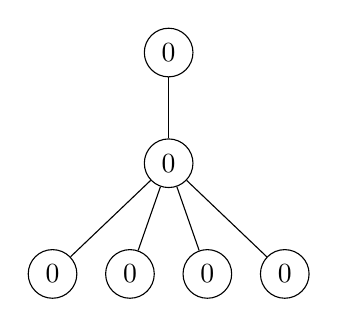
\begin{tikzpicture}[every tree node/.style={draw,circle},sibling distance=10pt, level distance=40pt]
\tikzset{edge from parent/.style={draw, edge from parent path=
{(\tikzparentnode) -- (\tikzchildnode)}}}
\Tree[.0 [.0 [.0 ] [.0 ] [.0 ] [.0 ] ] ] 
\end{tikzpicture}

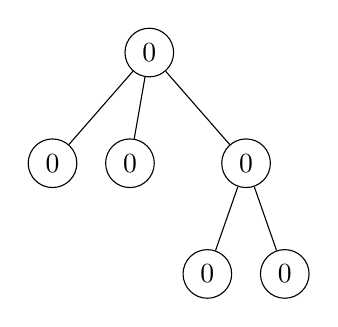
\begin{tikzpicture}[every tree node/.style={draw,circle},sibling distance=10pt, level distance=40pt]
\tikzset{edge from parent/.style={draw, edge from parent path=
{(\tikzparentnode) -- (\tikzchildnode)}}}
\Tree[.0 [.0 ] [.0 ] [.0 [.0 ] [.0 ] ] ] 
\end{tikzpicture}

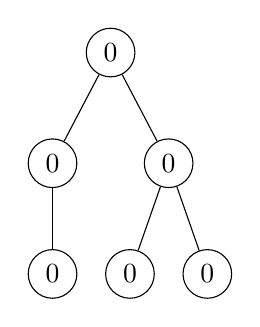
\begin{tikzpicture}[every tree node/.style={draw,circle},sibling distance=10pt, level distance=40pt]
\tikzset{edge from parent/.style={draw, edge from parent path=
{(\tikzparentnode) -- (\tikzchildnode)}}}
\Tree[.0 [.0 [.0 ] ] [.0 [.0 ] [.0 ] ] ] 
\end{tikzpicture}

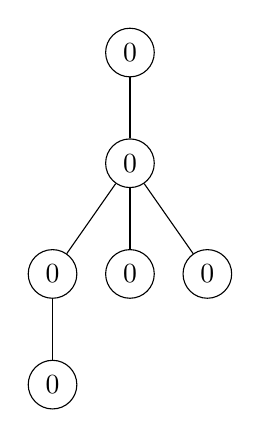
\begin{tikzpicture}[every tree node/.style={draw,circle},sibling distance=10pt, level distance=40pt]
\tikzset{edge from parent/.style={draw, edge from parent path=
{(\tikzparentnode) -- (\tikzchildnode)}}}
\Tree[.0 [.0 [.0 [.0 ] ] [.0 ] [.0 ] ] ] 
\end{tikzpicture}

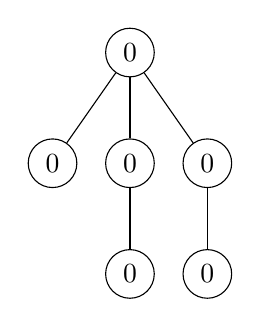
\begin{tikzpicture}[every tree node/.style={draw,circle},sibling distance=10pt, level distance=40pt]
\tikzset{edge from parent/.style={draw, edge from parent path=
{(\tikzparentnode) -- (\tikzchildnode)}}}
\Tree[.0 [.0 ] [.0 [.0 ] ] [.0 [.0 ] ] ] 
\end{tikzpicture}

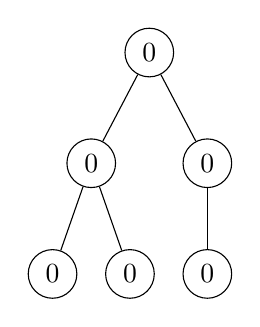
\begin{tikzpicture}[every tree node/.style={draw,circle},sibling distance=10pt, level distance=40pt]
\tikzset{edge from parent/.style={draw, edge from parent path=
{(\tikzparentnode) -- (\tikzchildnode)}}}
\Tree[.0 [.0 [.0 ] [.0 ] ] [.0 [.0 ] ] ] 
\end{tikzpicture}

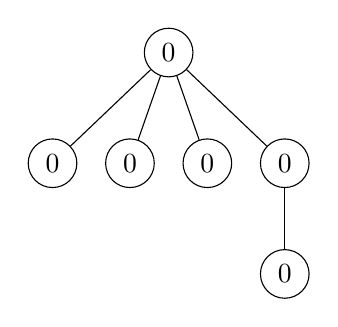
\begin{tikzpicture}[every tree node/.style={draw,circle},sibling distance=10pt, level distance=40pt]
\tikzset{edge from parent/.style={draw, edge from parent path=
{(\tikzparentnode) -- (\tikzchildnode)}}}
\Tree[.0 [.0 ] [.0 ] [.0 ] [.0 [.0 ] ] ] 
\end{tikzpicture}

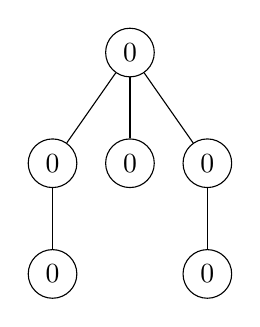
\begin{tikzpicture}[every tree node/.style={draw,circle},sibling distance=10pt, level distance=40pt]
\tikzset{edge from parent/.style={draw, edge from parent path=
{(\tikzparentnode) -- (\tikzchildnode)}}}
\Tree[.0 [.0 [.0 ] ] [.0 ] [.0 [.0 ] ] ] 
\end{tikzpicture}

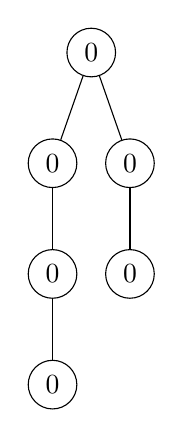
\begin{tikzpicture}[every tree node/.style={draw,circle},sibling distance=10pt, level distance=40pt]
\tikzset{edge from parent/.style={draw, edge from parent path=
{(\tikzparentnode) -- (\tikzchildnode)}}}
\Tree[.0 [.0 [.0 [.0 ] ] ] [.0 [.0 ] ] ] 
\end{tikzpicture}

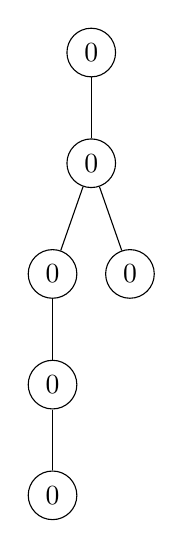
\begin{tikzpicture}[every tree node/.style={draw,circle},sibling distance=10pt, level distance=40pt]
\tikzset{edge from parent/.style={draw, edge from parent path=
{(\tikzparentnode) -- (\tikzchildnode)}}}
\Tree[.0 [.0 [.0 [.0 [.0 ] ] ] [.0 ] ] ] 
\end{tikzpicture}

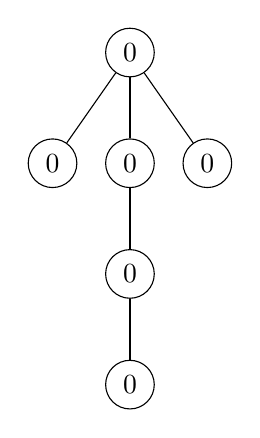
\begin{tikzpicture}[every tree node/.style={draw,circle},sibling distance=10pt, level distance=40pt]
\tikzset{edge from parent/.style={draw, edge from parent path=
{(\tikzparentnode) -- (\tikzchildnode)}}}
\Tree[.0 [.0 ] [.0 [.0 [.0 ] ] ] [.0 ] ] 
\end{tikzpicture}

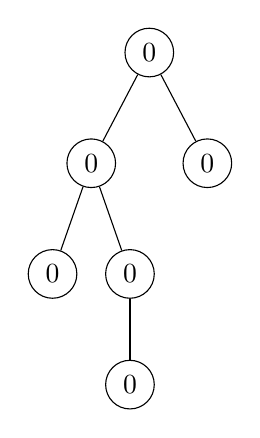
\begin{tikzpicture}[every tree node/.style={draw,circle},sibling distance=10pt, level distance=40pt]
\tikzset{edge from parent/.style={draw, edge from parent path=
{(\tikzparentnode) -- (\tikzchildnode)}}}
\Tree[.0 [.0 [.0 ] [.0 [.0 ] ] ] [.0 ] ] 
\end{tikzpicture}

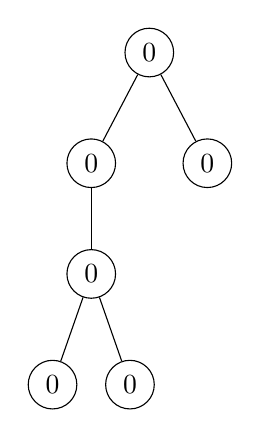
\begin{tikzpicture}[every tree node/.style={draw,circle},sibling distance=10pt, level distance=40pt]
\tikzset{edge from parent/.style={draw, edge from parent path=
{(\tikzparentnode) -- (\tikzchildnode)}}}
\Tree[.0 [.0 [.0 [.0 ] [.0 ] ] ] [.0 ] ] 
\end{tikzpicture}

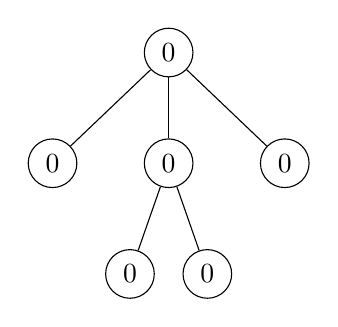
\begin{tikzpicture}[every tree node/.style={draw,circle},sibling distance=10pt, level distance=40pt]
\tikzset{edge from parent/.style={draw, edge from parent path=
{(\tikzparentnode) -- (\tikzchildnode)}}}
\Tree[.0 [.0 ] [.0 [.0 ] [.0 ] ] [.0 ] ] 
\end{tikzpicture}

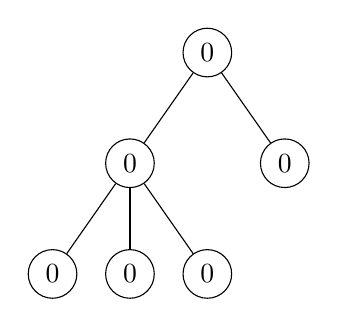
\begin{tikzpicture}[every tree node/.style={draw,circle},sibling distance=10pt, level distance=40pt]
\tikzset{edge from parent/.style={draw, edge from parent path=
{(\tikzparentnode) -- (\tikzchildnode)}}}
\Tree[.0 [.0 [.0 ] [.0 ] [.0 ] ] [.0 ] ] 
\end{tikzpicture}

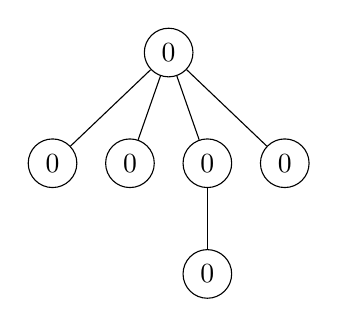
\begin{tikzpicture}[every tree node/.style={draw,circle},sibling distance=10pt, level distance=40pt]
\tikzset{edge from parent/.style={draw, edge from parent path=
{(\tikzparentnode) -- (\tikzchildnode)}}}
\Tree[.0 [.0 ] [.0 ] [.0 [.0 ] ] [.0 ] ] 
\end{tikzpicture}

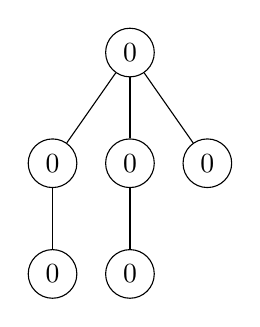
\begin{tikzpicture}[every tree node/.style={draw,circle},sibling distance=10pt, level distance=40pt]
\tikzset{edge from parent/.style={draw, edge from parent path=
{(\tikzparentnode) -- (\tikzchildnode)}}}
\Tree[.0 [.0 [.0 ] ] [.0 [.0 ] ] [.0 ] ] 
\end{tikzpicture}

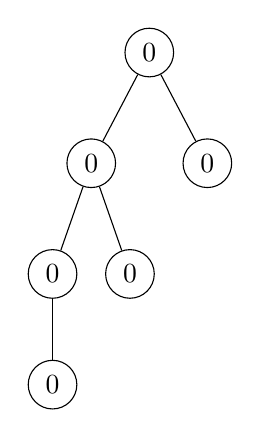
\begin{tikzpicture}[every tree node/.style={draw,circle},sibling distance=10pt, level distance=40pt]
\tikzset{edge from parent/.style={draw, edge from parent path=
{(\tikzparentnode) -- (\tikzchildnode)}}}
\Tree[.0 [.0 [.0 [.0 ] ] [.0 ] ] [.0 ] ] 
\end{tikzpicture}

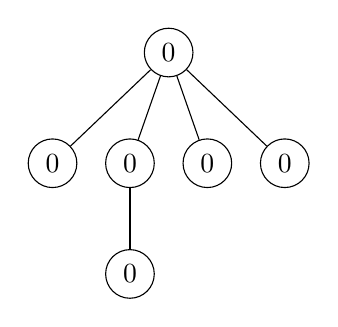
\begin{tikzpicture}[every tree node/.style={draw,circle},sibling distance=10pt, level distance=40pt]
\tikzset{edge from parent/.style={draw, edge from parent path=
{(\tikzparentnode) -- (\tikzchildnode)}}}
\Tree[.0 [.0 ] [.0 [.0 ] ] [.0 ] [.0 ] ] 
\end{tikzpicture}

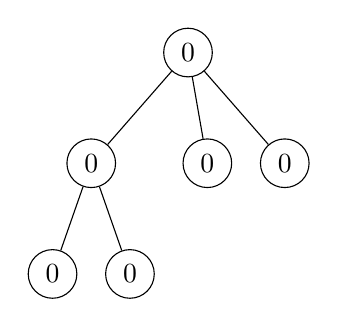
\begin{tikzpicture}[every tree node/.style={draw,circle},sibling distance=10pt, level distance=40pt]
\tikzset{edge from parent/.style={draw, edge from parent path=
{(\tikzparentnode) -- (\tikzchildnode)}}}
\Tree[.0 [.0 [.0 ] [.0 ] ] [.0 ] [.0 ] ] 
\end{tikzpicture}

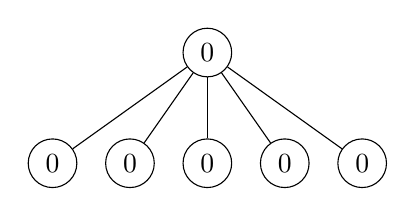
\begin{tikzpicture}[every tree node/.style={draw,circle},sibling distance=10pt, level distance=40pt]
\tikzset{edge from parent/.style={draw, edge from parent path=
{(\tikzparentnode) -- (\tikzchildnode)}}}
\Tree[.0 [.0 ] [.0 ] [.0 ] [.0 ] [.0 ] ] 
\end{tikzpicture}

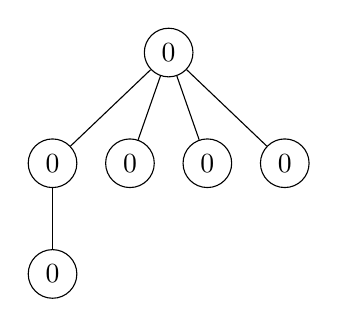
\begin{tikzpicture}[every tree node/.style={draw,circle},sibling distance=10pt, level distance=40pt]
\tikzset{edge from parent/.style={draw, edge from parent path=
{(\tikzparentnode) -- (\tikzchildnode)}}}
\Tree[.0 [.0 [.0 ] ] [.0 ] [.0 ] [.0 ] ] 
\end{tikzpicture}

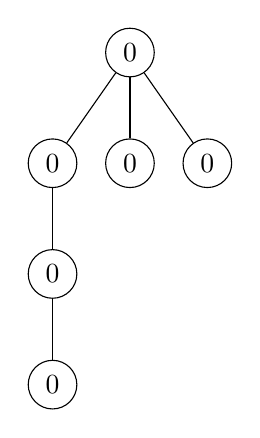
\begin{tikzpicture}[every tree node/.style={draw,circle},sibling distance=10pt, level distance=40pt]
\tikzset{edge from parent/.style={draw, edge from parent path=
{(\tikzparentnode) -- (\tikzchildnode)}}}
\Tree[.0 [.0 [.0 [.0 ] ] ] [.0 ] [.0 ] ] 
\end{tikzpicture}

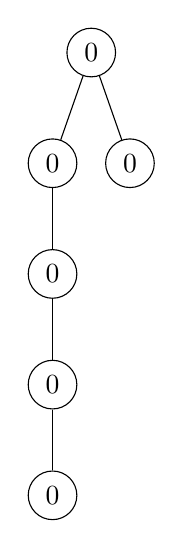
\begin{tikzpicture}[every tree node/.style={draw,circle},sibling distance=10pt, level distance=40pt]
\tikzset{edge from parent/.style={draw, edge from parent path=
{(\tikzparentnode) -- (\tikzchildnode)}}}
\Tree[.0 [.0 [.0 [.0 [.0 ] ] ] ] [.0 ] ] 
\end{tikzpicture}

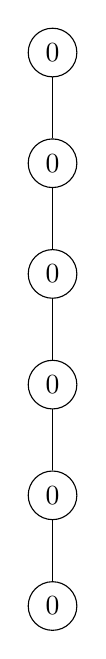
\begin{tikzpicture}[every tree node/.style={draw,circle},sibling distance=10pt, level distance=40pt]
\tikzset{edge from parent/.style={draw, edge from parent path=
{(\tikzparentnode) -- (\tikzchildnode)}}}
\Tree[.0 [.0 [.0 [.0 [.0 [.0 ] ] ] ] ] ] 
\end{tikzpicture}


\end{document}
